\documentclass{article}
%\usepackage{fullpage}
%\usepackage{fullpage}
\usepackage{amsmath}
\usepackage{latexsym}
\usepackage{amssymb,amsfonts}
\usepackage{graphicx}
\usepackage{graphics}
\usepackage[margin=.75in]{geometry}

\begin{document}

\phantom{.}\hspace{-.5in}\begin{tabular}{lr}
 \begin{tabular}{l}
    
\includegraphics[width=2in]{AUExploreLogo.pdf}
 \end{tabular}
 & \hspace{.5in}
 \begin{tabular}{r}
    {\Huge Attacking Board Game}
 \end{tabular}
\end{tabular}
\thispagestyle{empty}

\noindent\hrulefill
\phantom{.}\vspace{.15in}

{\Large
\begin{enumerate}
\item Place eight blue pieces on the board. Blue pieces are able to attack any square which is dirrectly vertical or horizontal from its location.
\begin{figure}[h]
\begin{center}
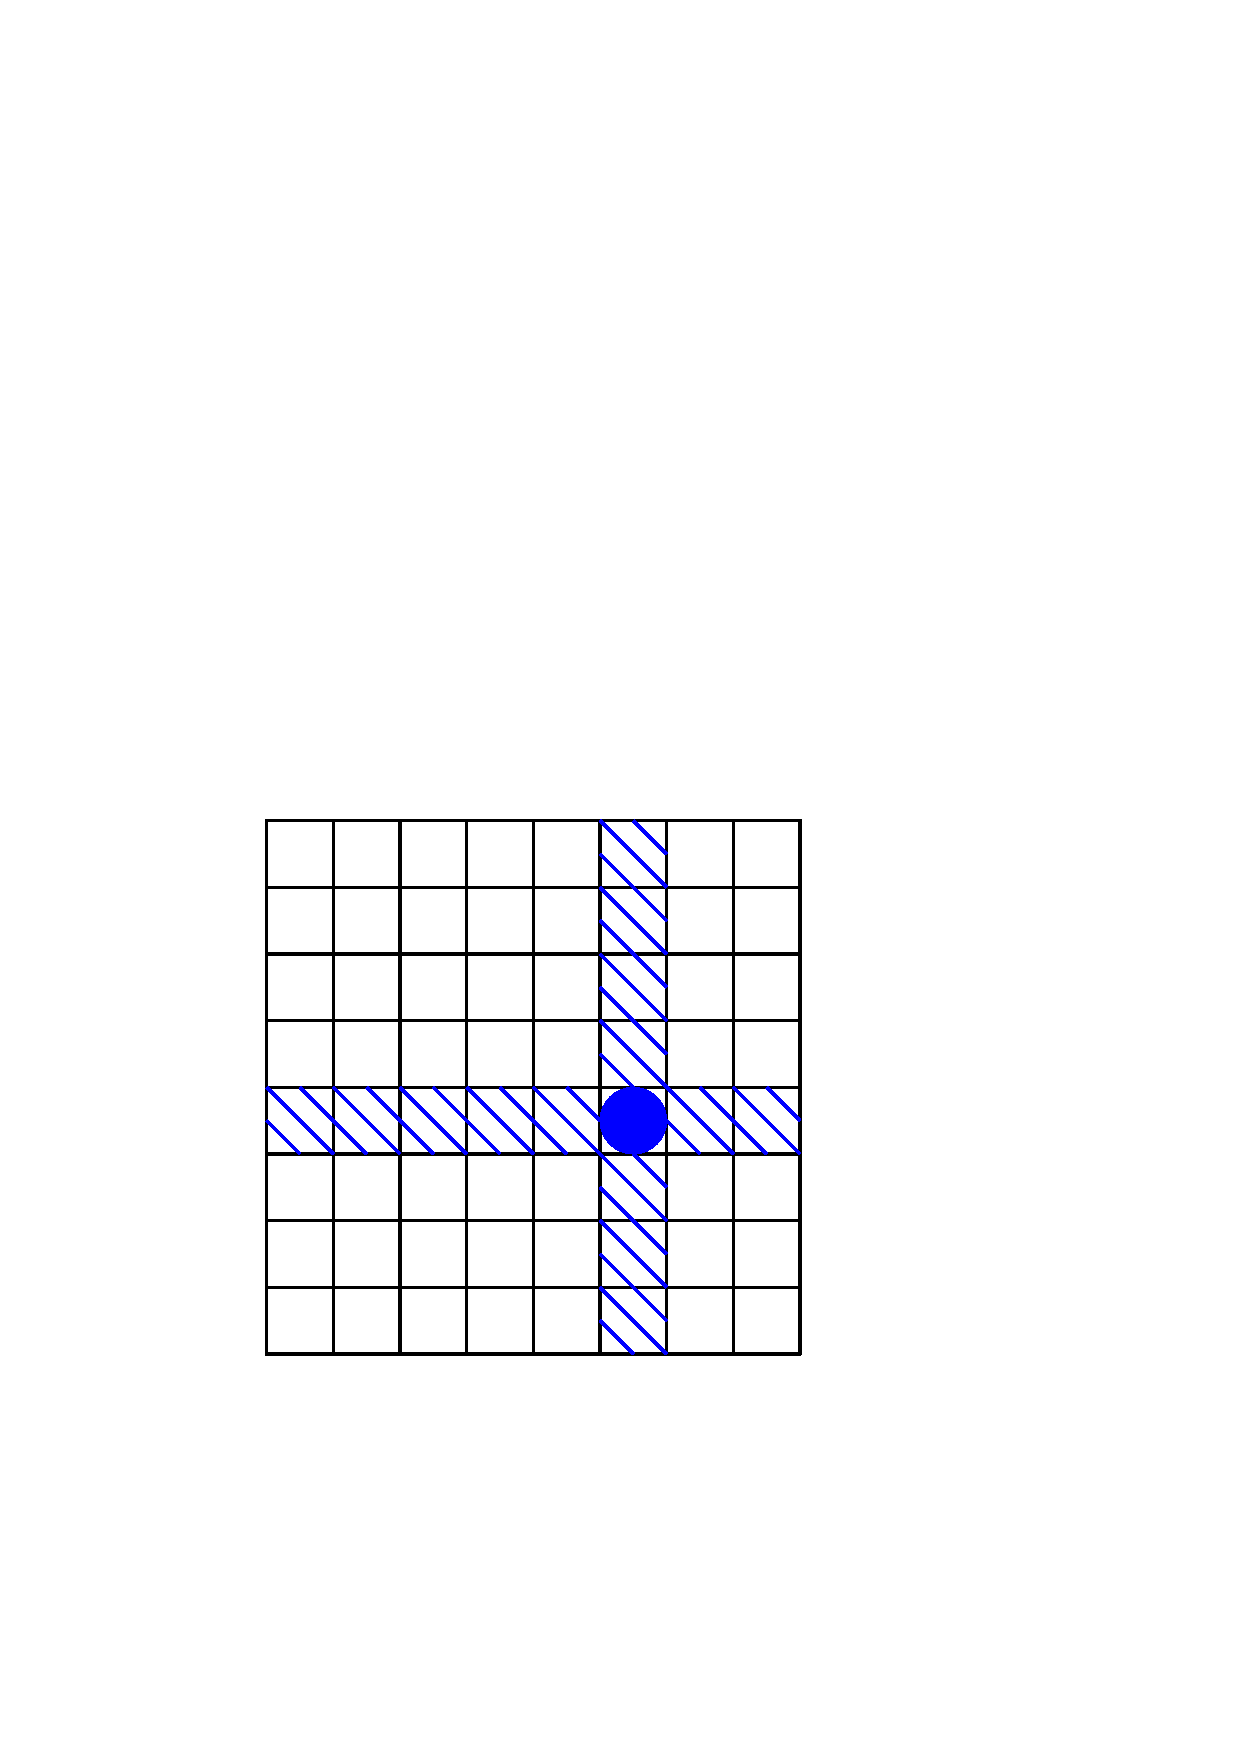
\includegraphics[width=1.3in]{RookAttack.pdf}
\end{center}
\end{figure}
\item Place eight orange pieces on the board. Orange pieces are able to attack any square which is is located on a diagonal containing its location.
\begin{figure}[h]
\begin{center}
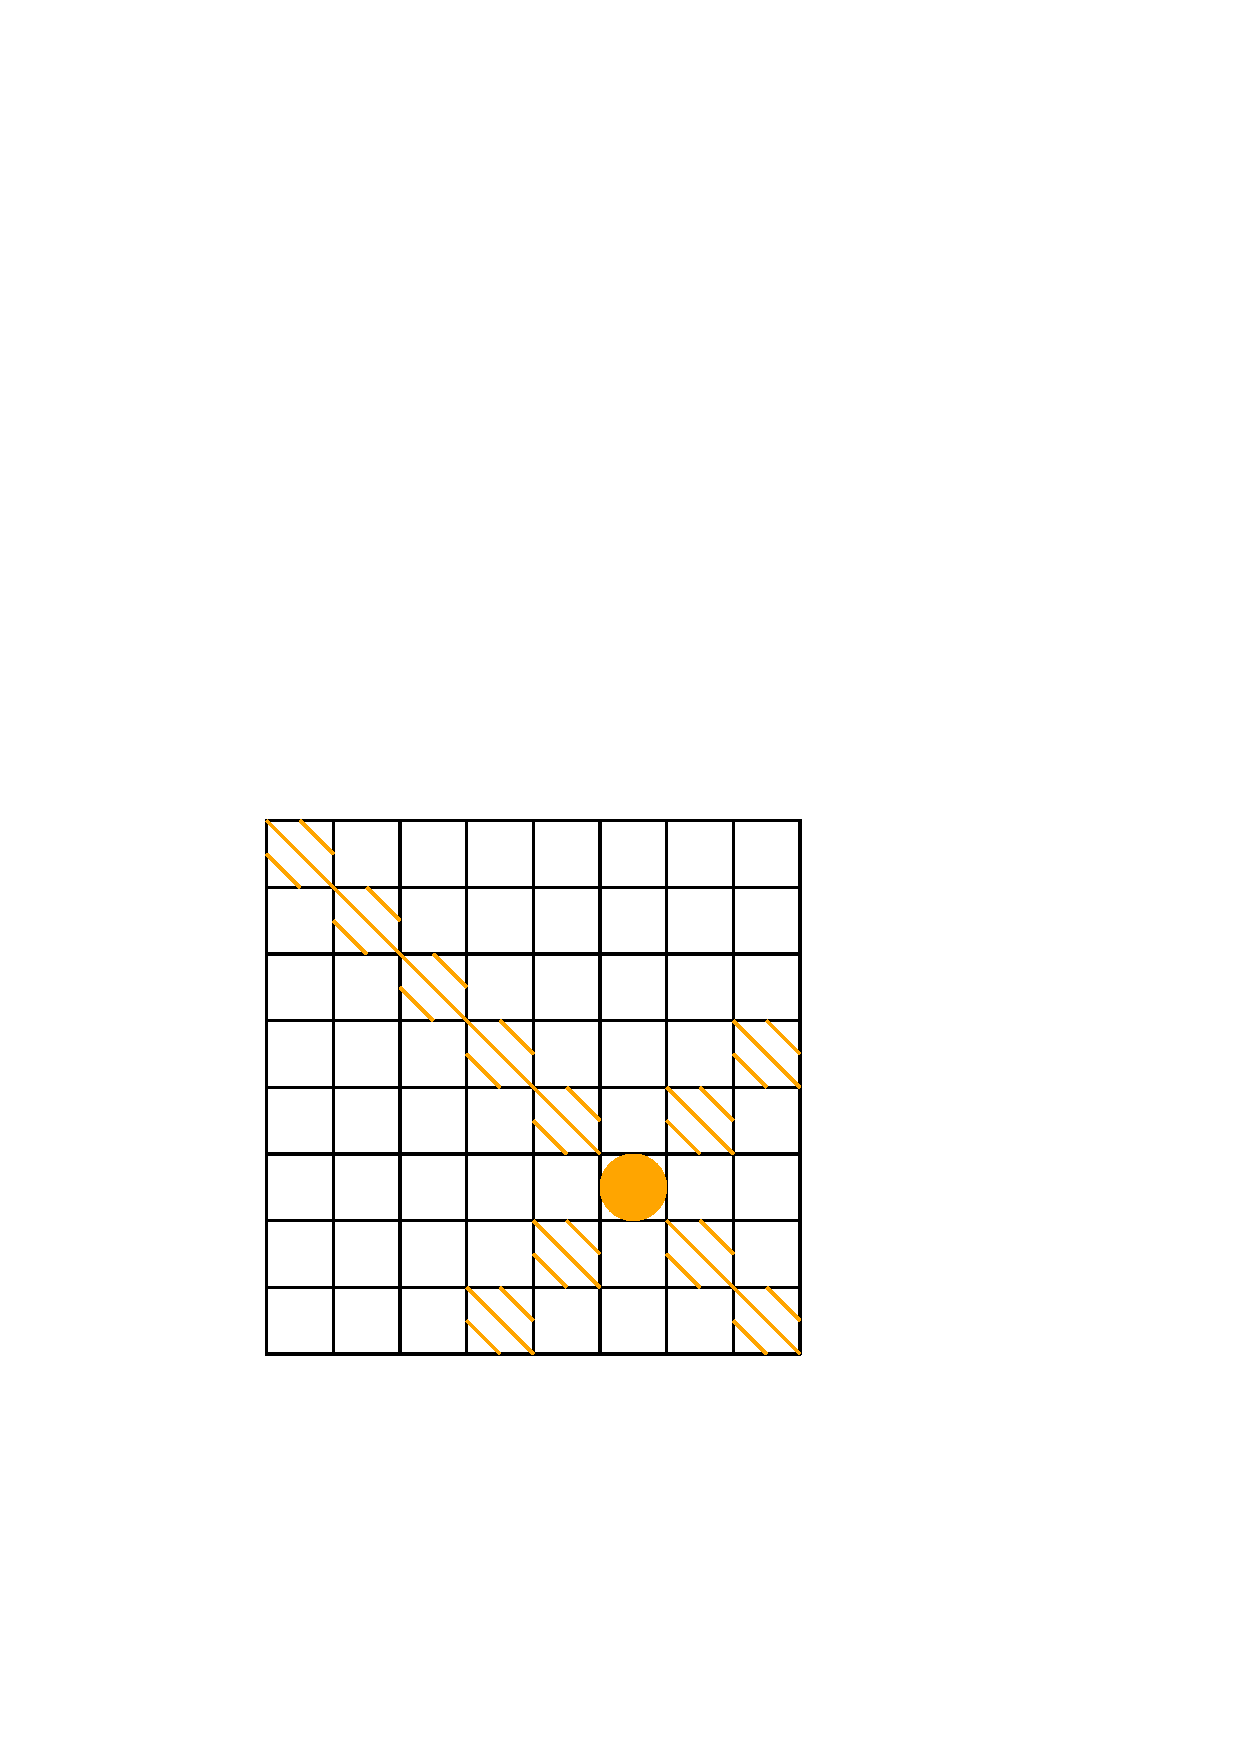
\includegraphics[width=1.3in]{BishopAttack.pdf}
\end{center}
\end{figure}
\item Place eight green pieces on the board. Green pieces are able to attack any square which could be attacked by a Blue piece or an Orange piece.
\begin{figure}[h]
\begin{center}
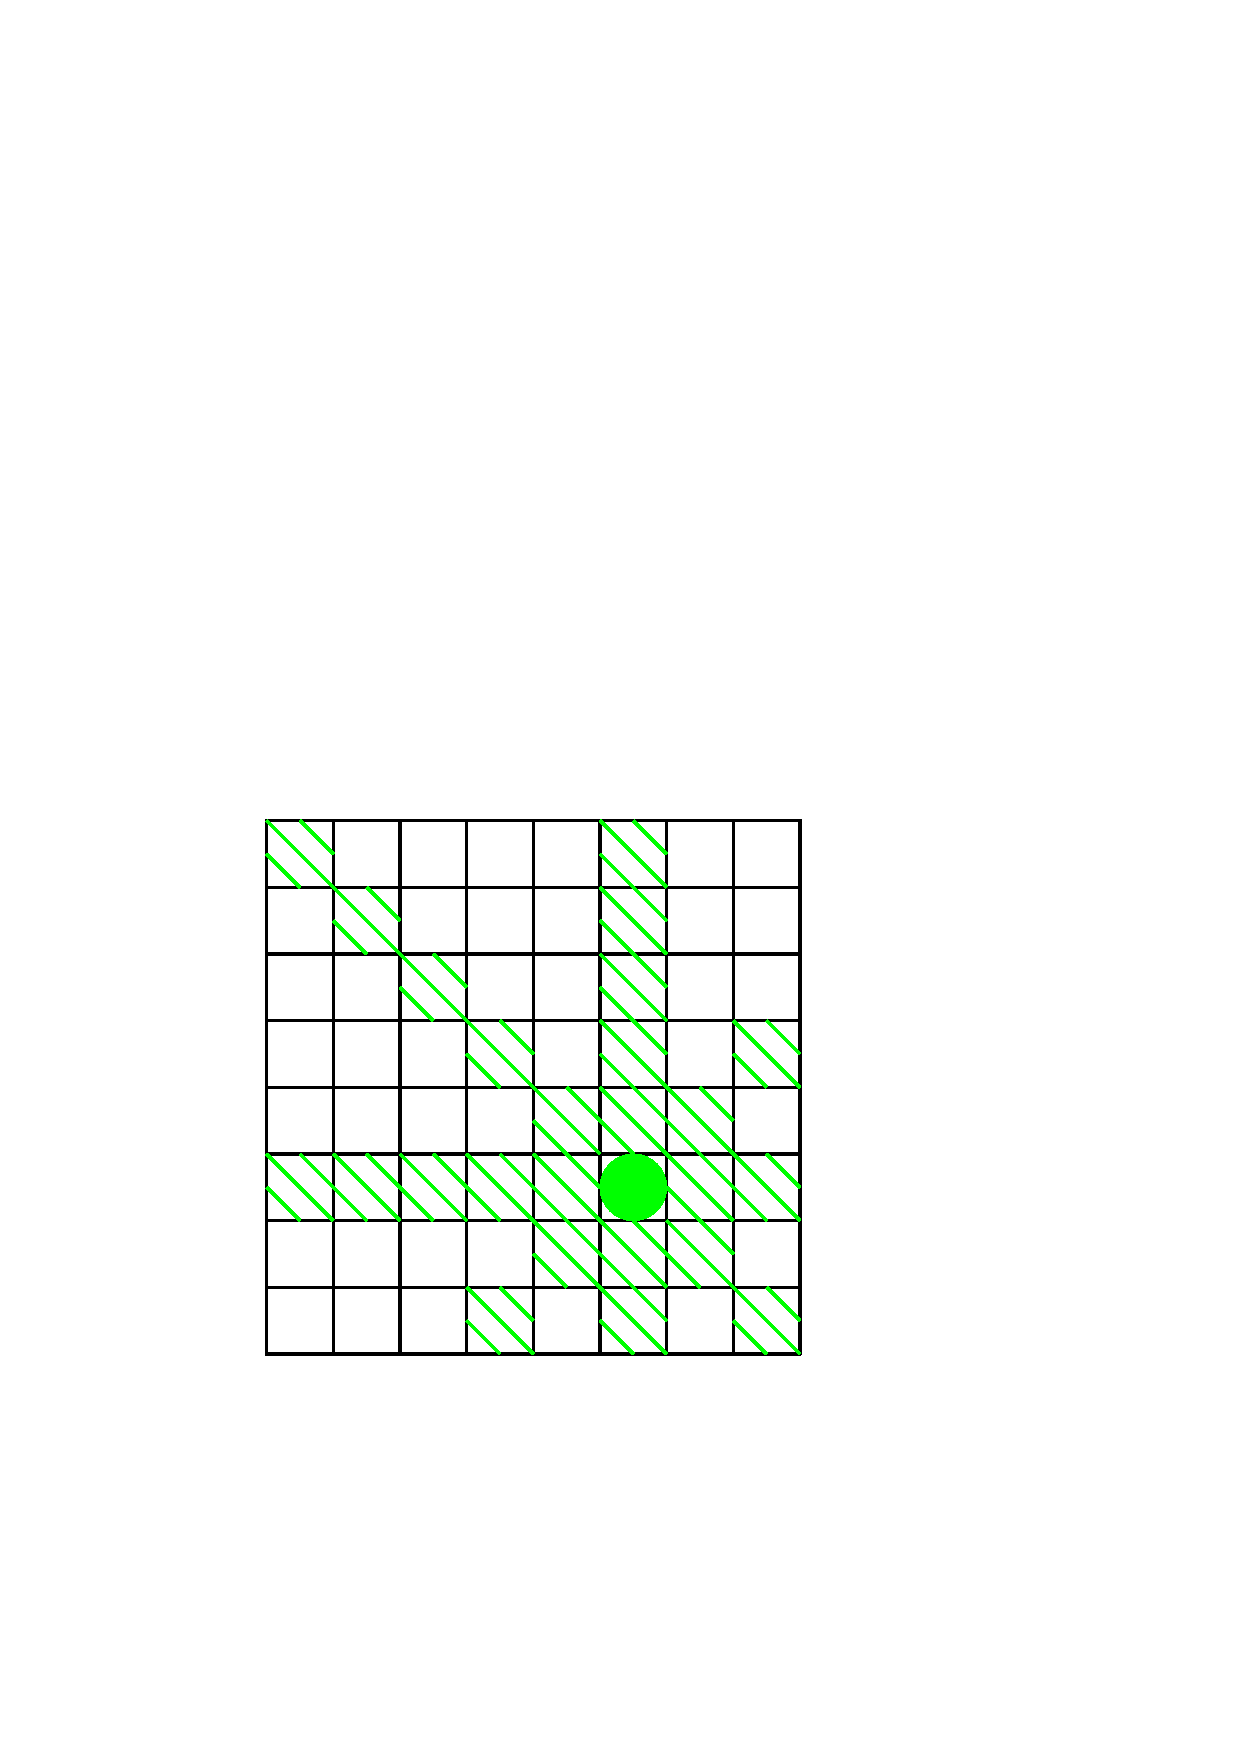
\includegraphics[width=1.3in]{QueenAttack.pdf}
\end{center}
\end{figure}
\end{enumerate}
\end{document}
